
\chapter{Introduction} \label{Chap: introduction}

This is a latex template for Ph.D. thesis in The Hong Kong Polytechnic University. It can be also used for other universities or degrees.

\section{Commands}

This is an example for renew commands, \eg, we can use \textbackslash eg to generate \eg. The same thing goes to \etc.

We can use \textbackslash rev\{\} to mark your text: \rev{revised text}. 


\section{Citation}

This is an example for citation \cite{pan2012investigation}.

\section{Figures}


This is a figure, as shown in \fref{fig:figure}.


 \begin{figure}[t]
     \centering
     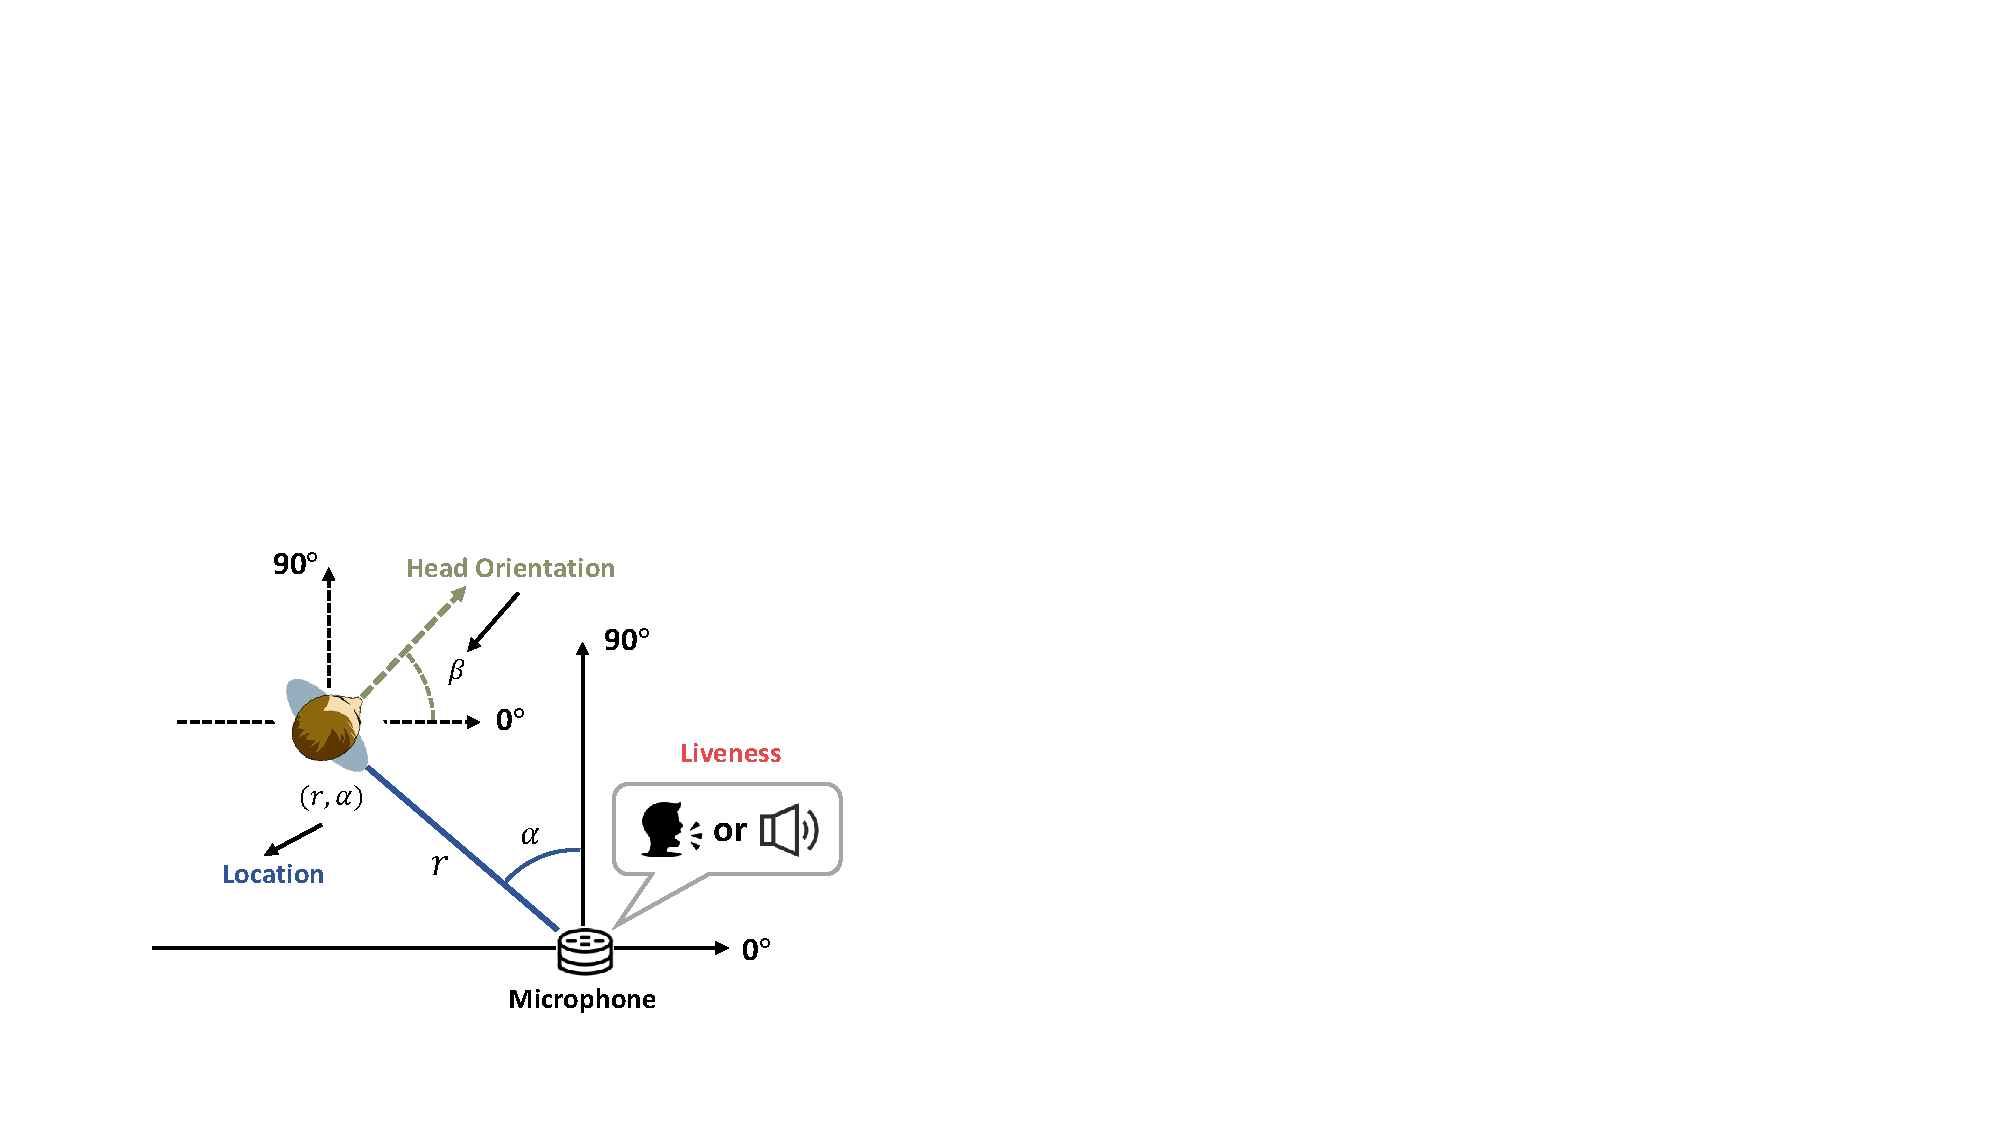
\includegraphics[width=0.5\textwidth]{Figures/Illustration.pdf}
     \caption{Illustration of a figure.}
     \label{fig:figure}
 \end{figure}

Figure \ref{fig:subfigure} shows an example of subfigures (\fref{fig:subfigure1} and \fref{fig:subfigure2}).


\begin{figure}[t]
\centering
\subfloat[Subfigure 1]{
		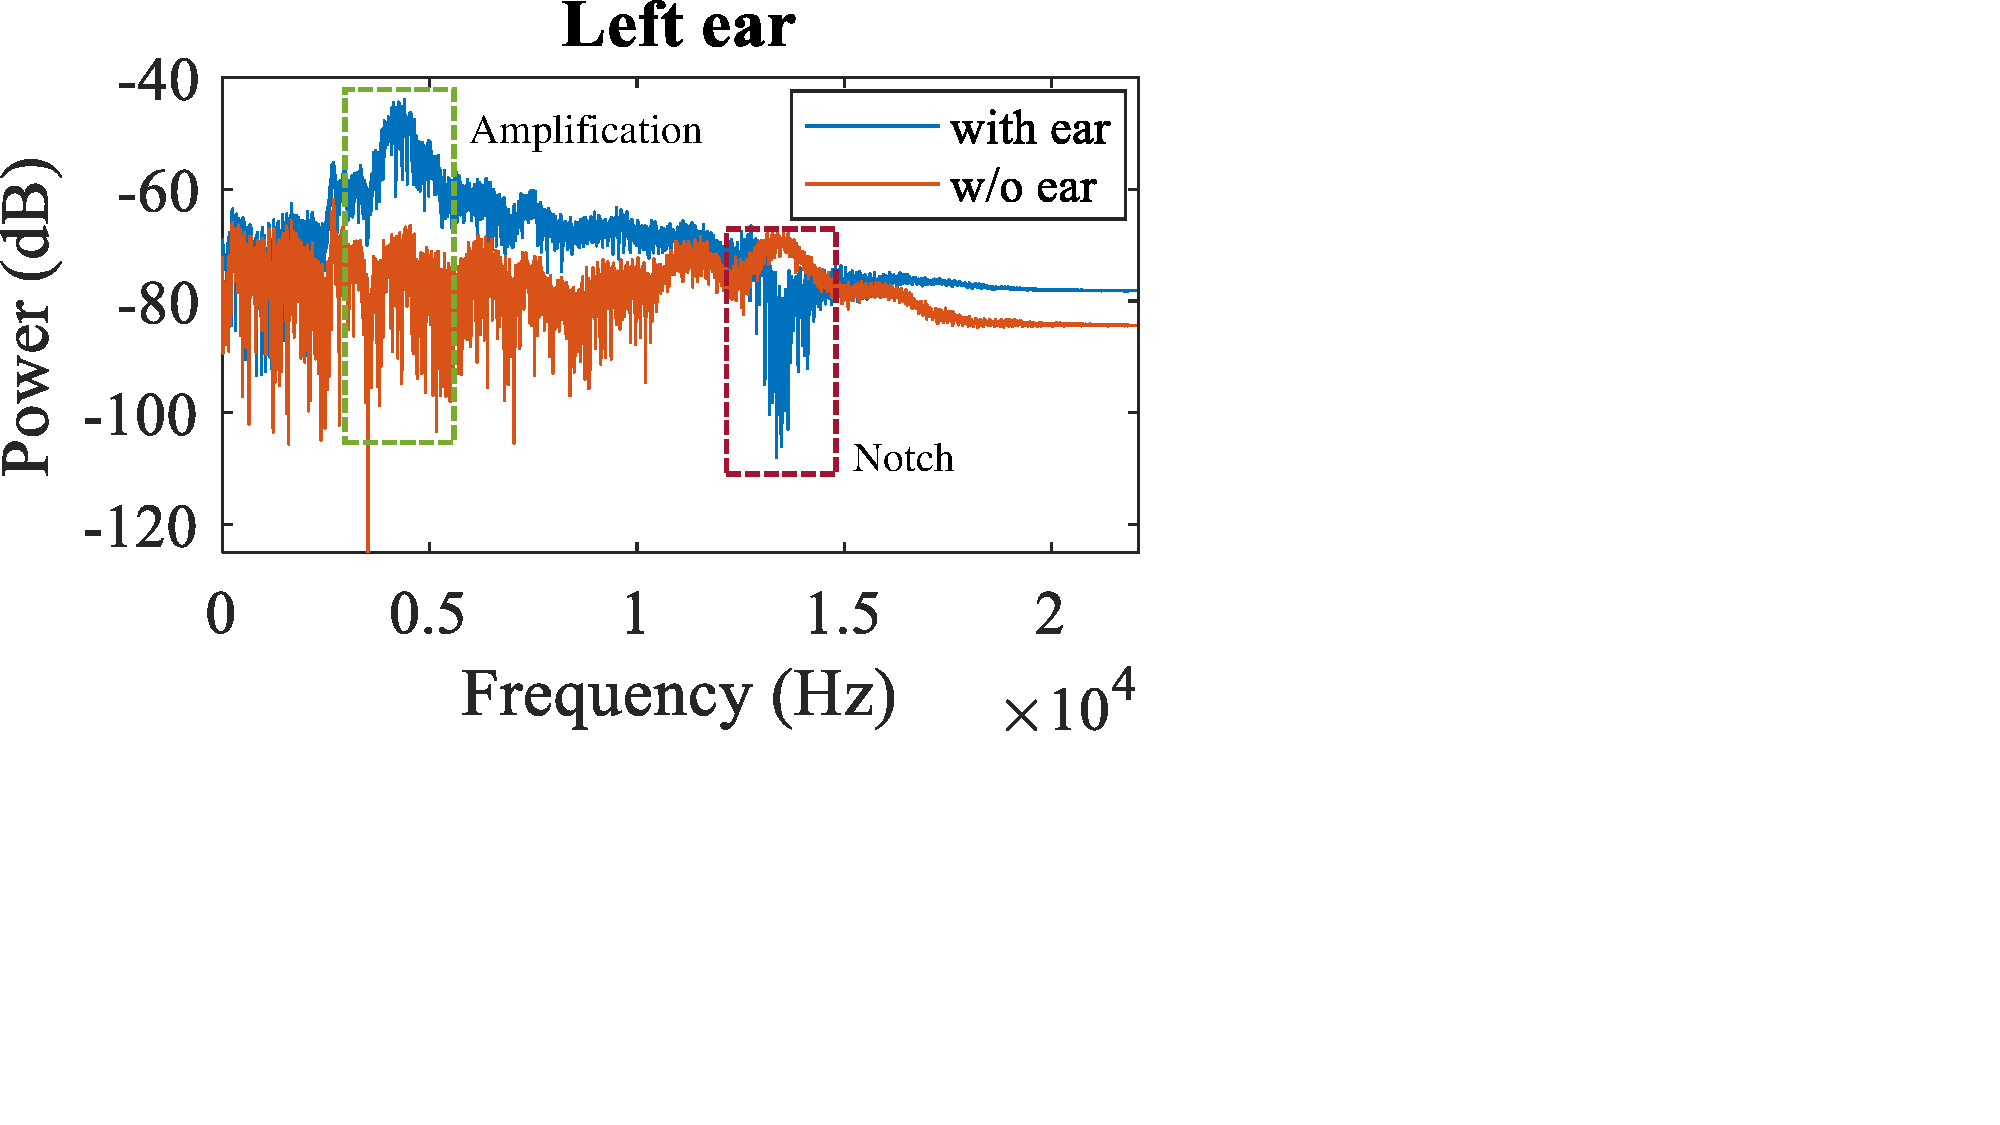
\includegraphics[width=0.45\columnwidth]{Figures/fr_ear_left.pdf} 
		\label{fig:subfigure1}
	}
\subfloat[Subfigure 2]{
		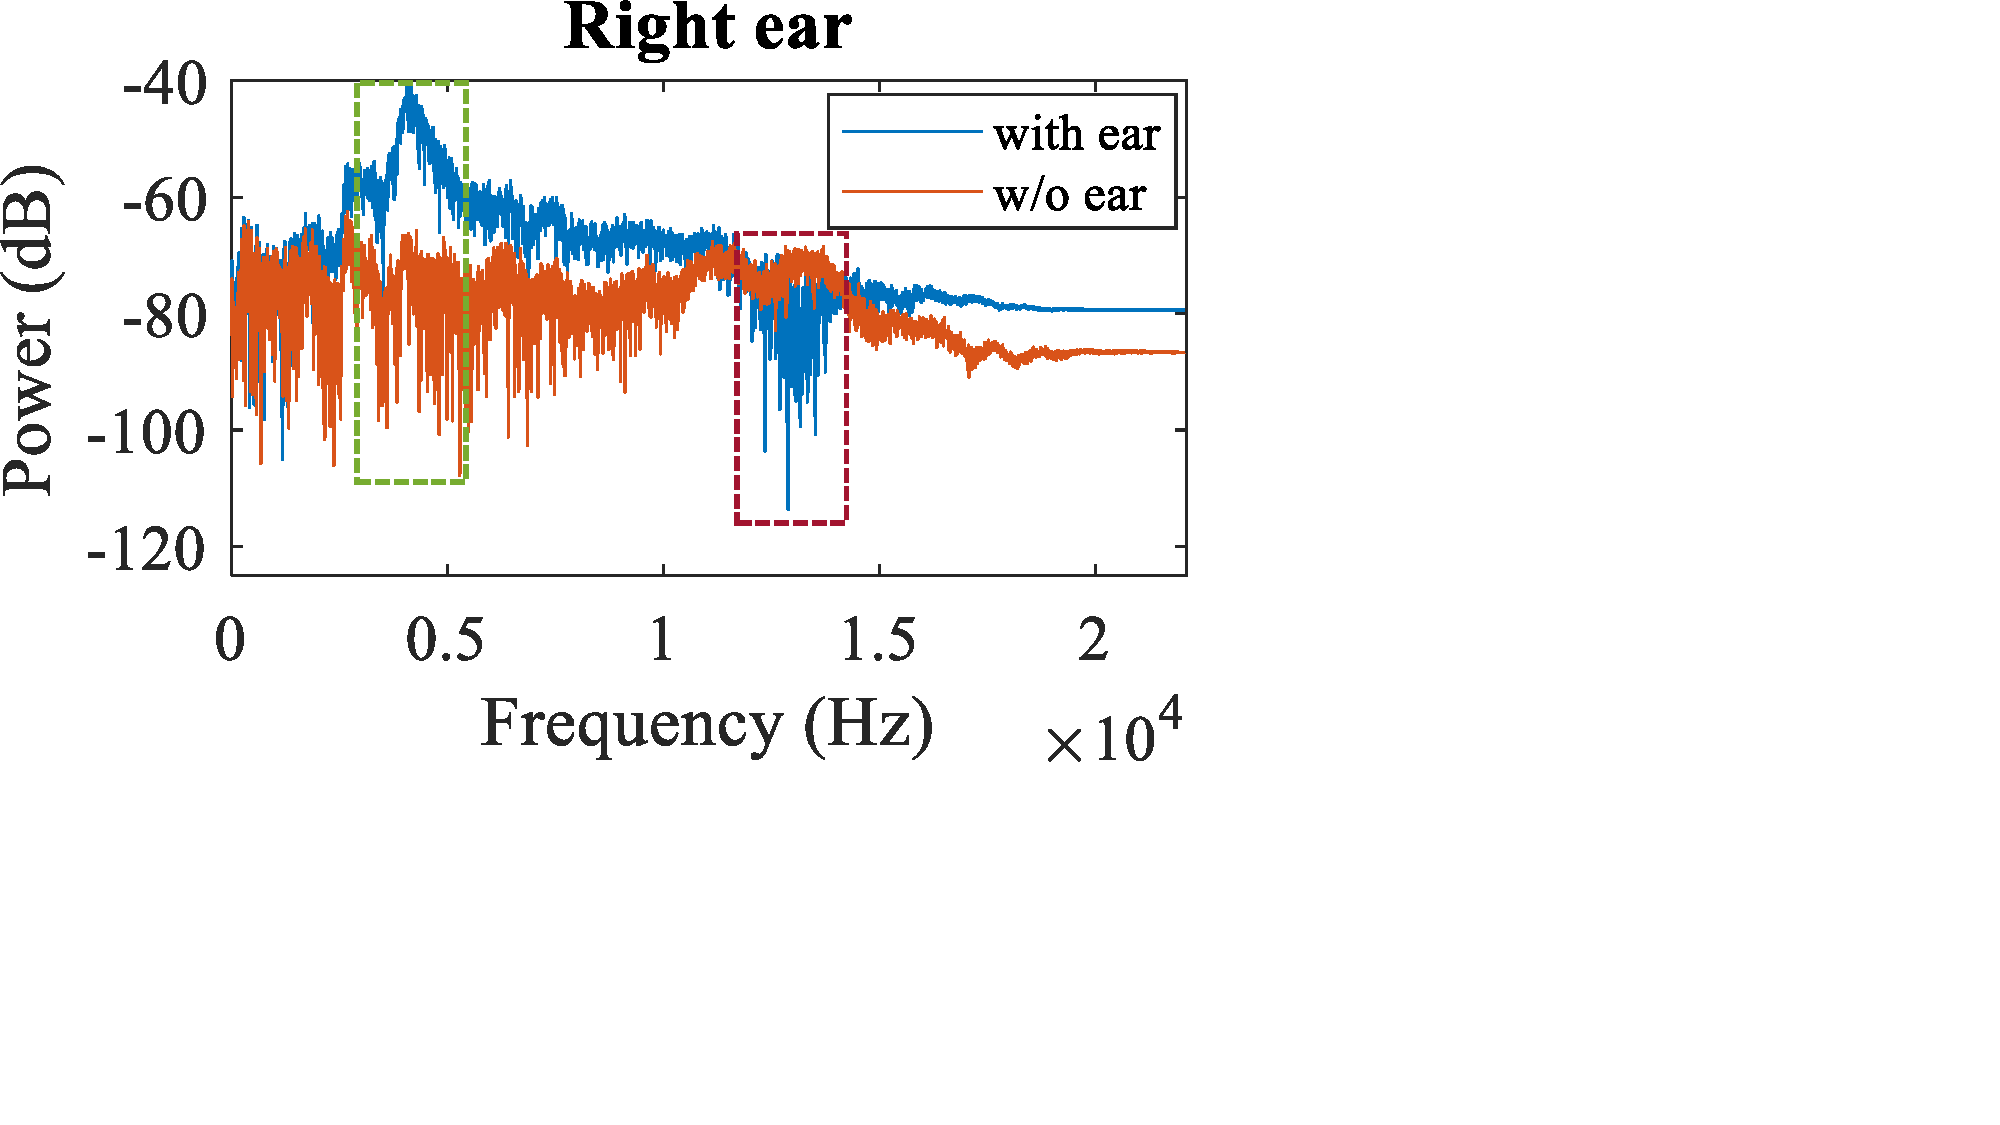
\includegraphics[width=0.45\columnwidth]{Figures/fr_ear_right.pdf}
		\label{fig:subfigure2}
	}
\caption{Frequency response with and without ears.}
\label{fig:subfigure}
\end{figure}


This is an example for the minipage (\fref{fig:minipage1} and \fref{fig:minipage2}).

\begin{figure}[t]
\begin{minipage}{0.48\linewidth}
        \centering
		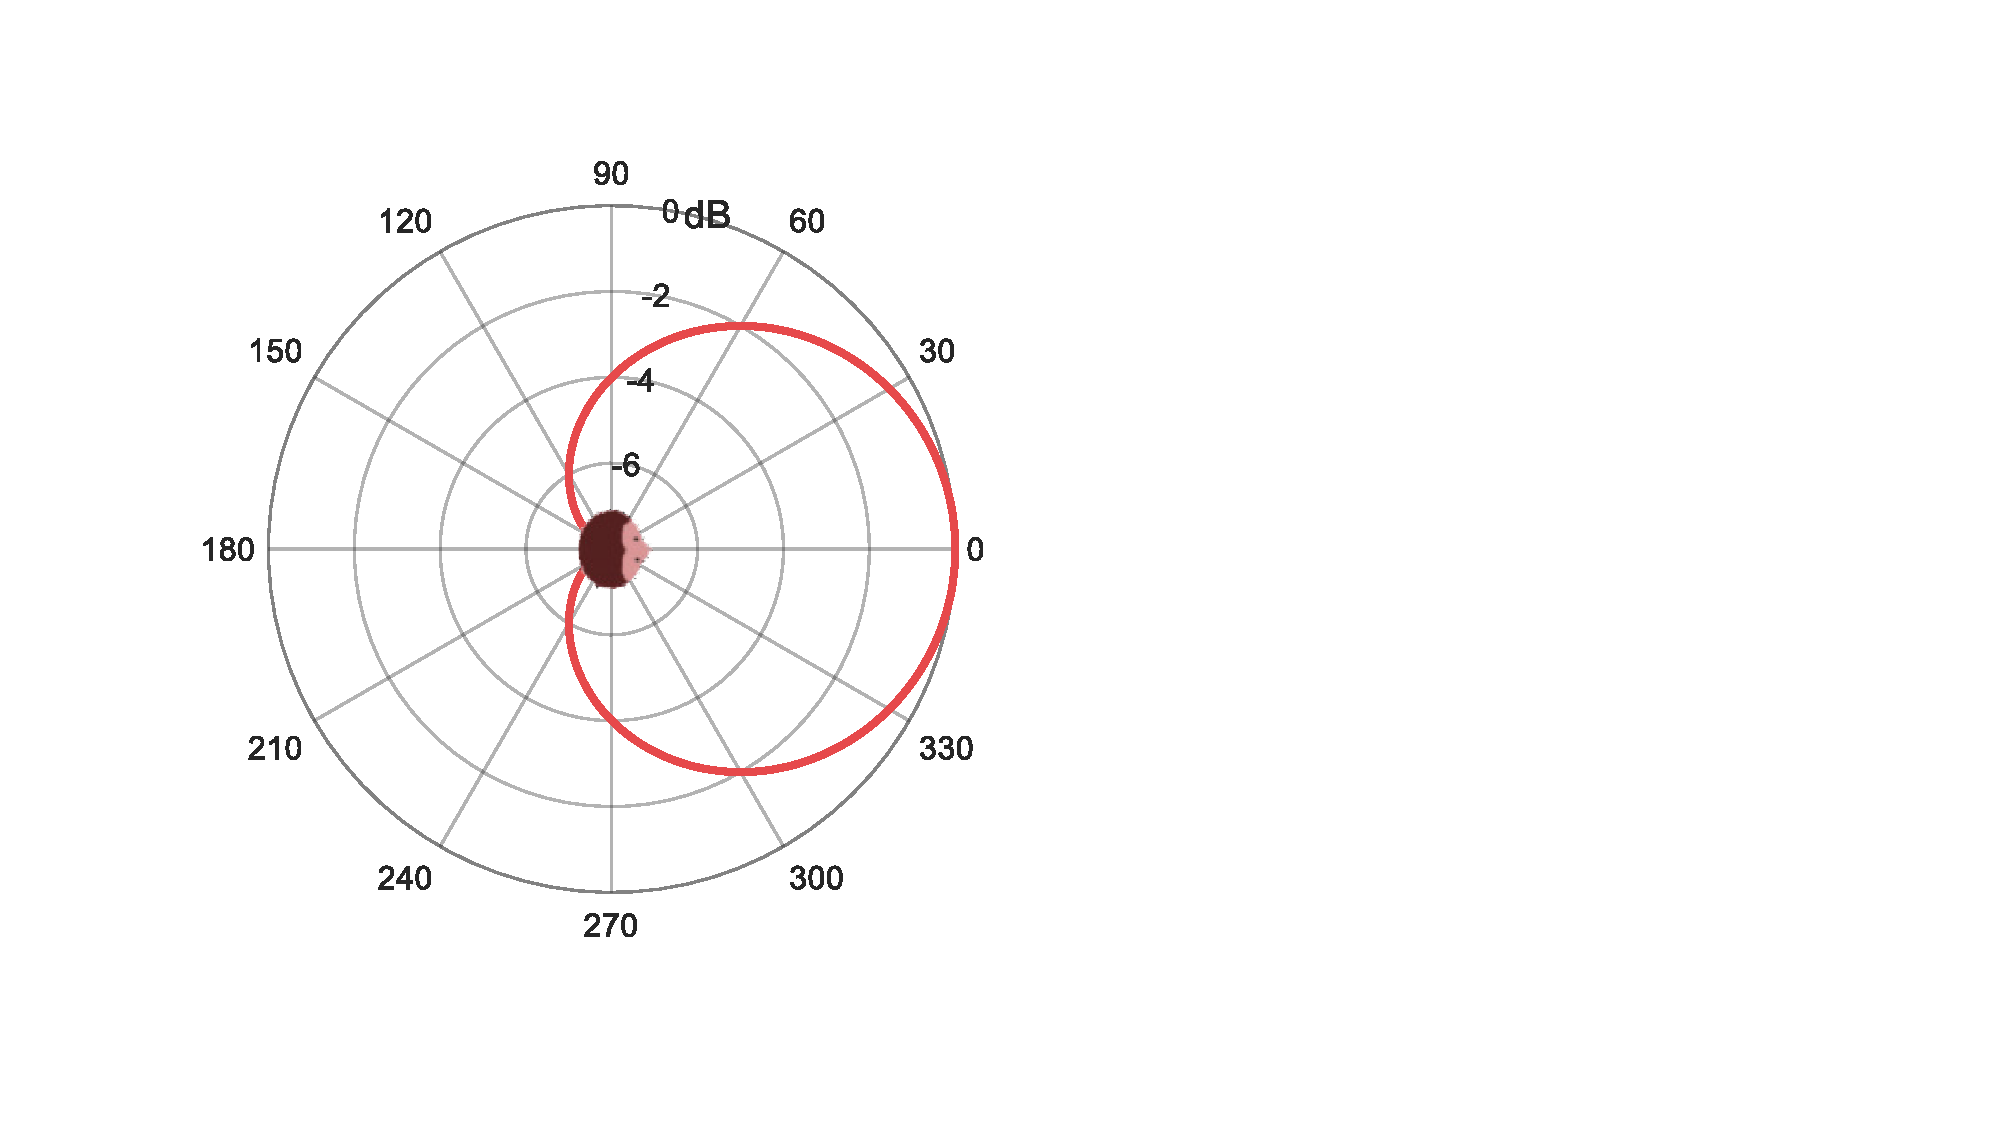
\includegraphics[width=0.58\columnwidth]{Figures/OE_cardioid.pdf}
		\caption{Minipage 1.}
		\label{fig:minipage1}
\end{minipage}
\hspace{5pt}
\begin{minipage}{0.48\linewidth}
        \centering
		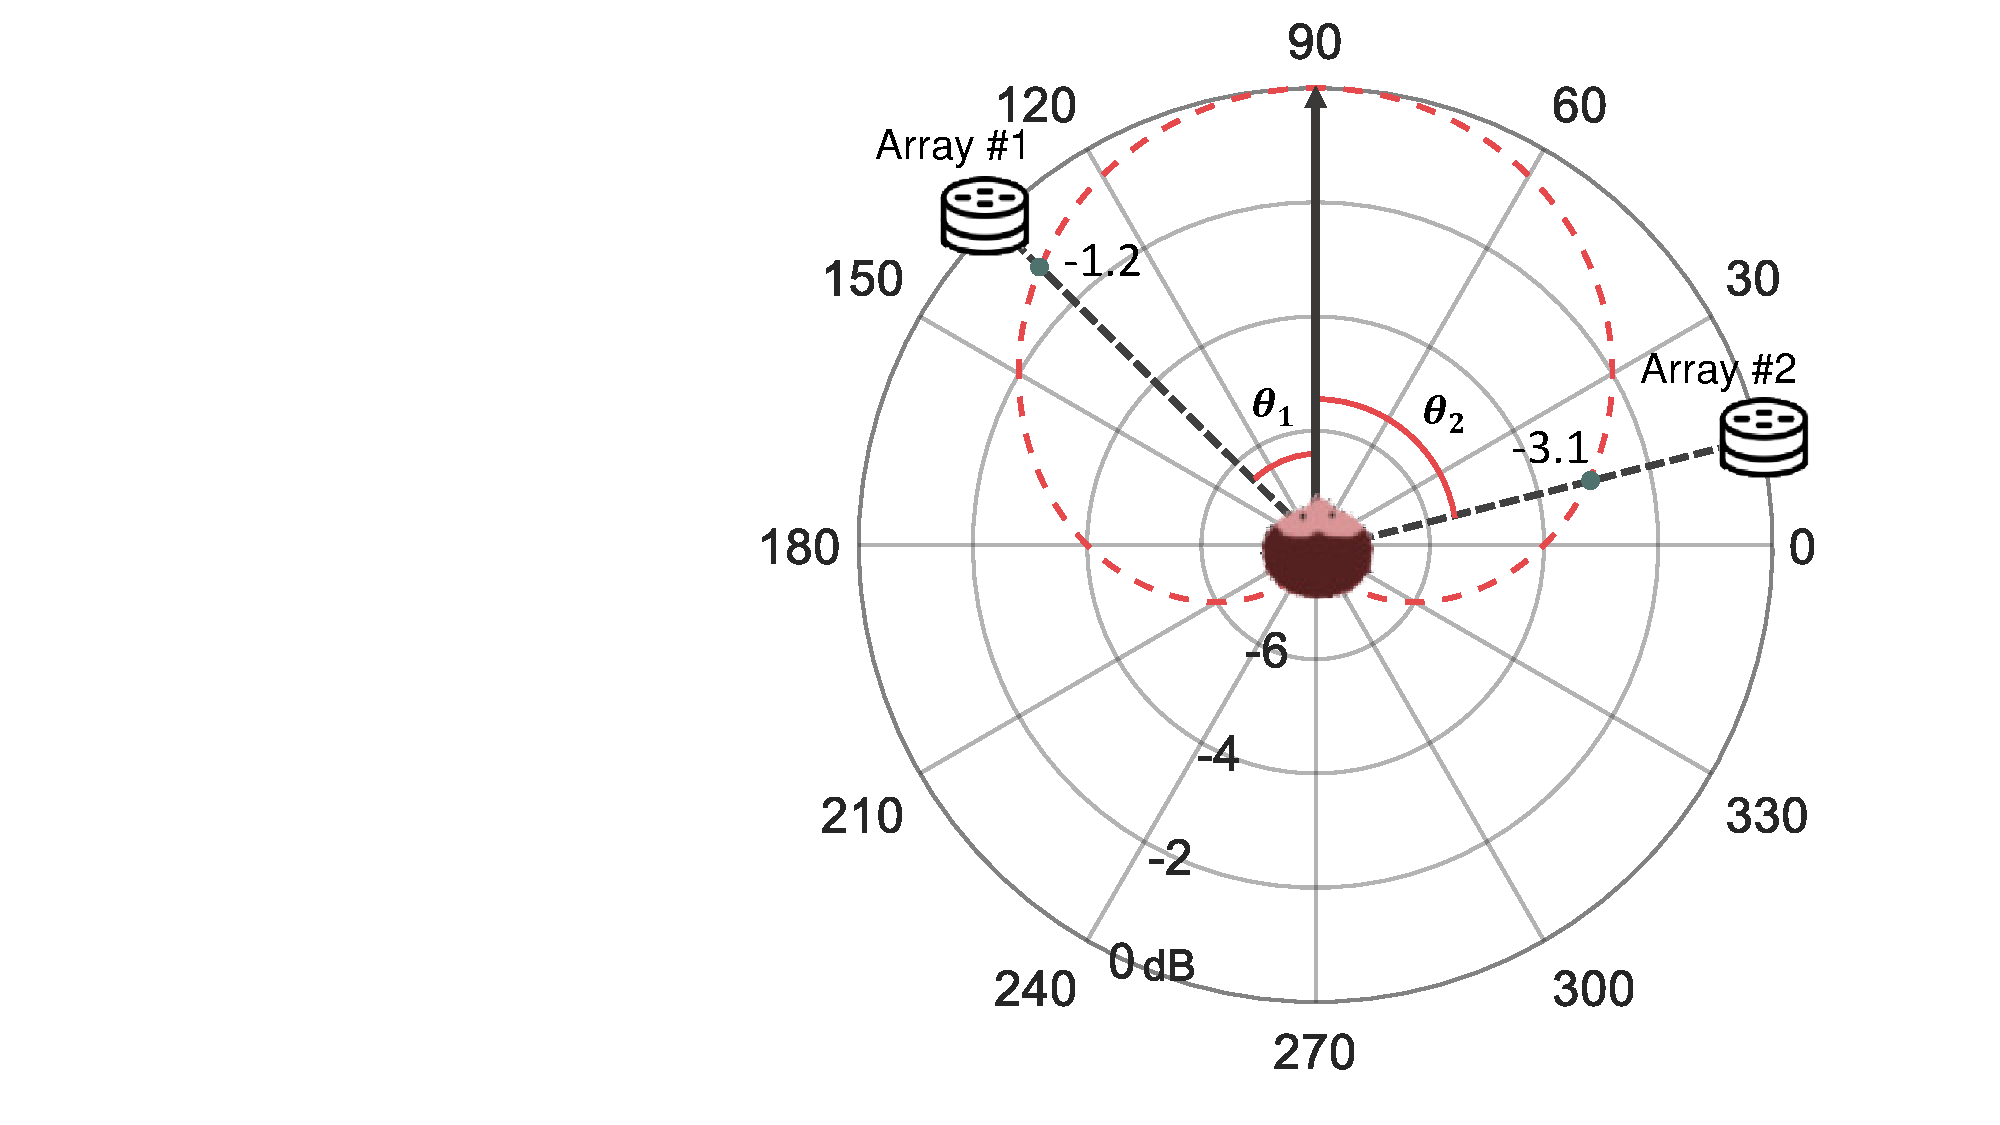
\includegraphics[width=0.58\columnwidth]{OE_sameDisDiffDeg.pdf}
		\caption{Minipage 2.}
		\label{fig:minipage2}
\end{minipage}
\end{figure}

\section{Table}


A table example is shown in \tref{tab:table}. It is a three-line table.


\begin{table}[t]
\renewcommand{\arraystretch}{1.1}
\centering
\caption{PolyU rankings.}
\begin{tabular}{ccccc}
\toprule
Rankings &
  \begin{tabular}[c]{@{}c@{}}QS \\ World University\end{tabular} &
  \begin{tabular}[c]{@{}c@{}}QS \\ Asia University \end{tabular} &
  \begin{tabular}[c]{@{}c@{}}THE \\ World University \end{tabular} &
  \begin{tabular}[c]{@{}c@{}}THE \\ Asia University\end{tabular} \\ \midrule
2022 &
  66 &
  25 &
  91 &
  15 \\ 
2021 &
  75 &
  25 &
  129 &
  23 \\ \bottomrule
\end{tabular}
\vspace{10pt}
\label{tab:table}
\end{table}

\section{Examples}


\kant[1-3]